% by Mirella M. Moro; version: January/18/2012 @ 04:16pm
% -- 01/18/2012: more discussion on SBBD + kdmile; overall revision
% -- 09/03/2010: bib file with names for proceedings and journals; cls with shrinked {received}
% -- 08/27/2010: appendix, table example, more explanation within comments, editors' data

\documentclass[kdmile,a4paper]{kdmile} % NOTE: kdmile is published on A4 paper
\usepackage{graphicx,url}  % for using figures and url format
\usepackage{caption}
\usepackage{subcaption}
\usepackage[T1]{fontenc}   % avoids warnings such as "LaTeX Font Warning: Font shape 'OMS/cmtt/m/n' undefined"
\usepackage[brazilian]{babel}
\usepackage[usenames,dvipsnames]{color}
\usepackage{soul,xcolor}
\usepackage{algorithm}
\usepackage[noend]{algorithmic}
\usepackage{amsmath}
\usepackage[normalem]{ulem}

%\usepackage{cite} % NOTE: do **not** include this package because it conflicts with kdmile.bst

% Standard definitions
\newtheorem{theorem}{Theorem}[section]
\newtheorem{conjecture}[theorem]{Conjecture}
\newtheorem{corollary}[theorem]{Corollary}
\newtheorem{proposition}[theorem]{Proposition}
\newtheorem{lemma}[theorem]{Lemma}
\newdef{definition}[theorem]{Definition}
\newdef{remark}[theorem]{Remark}

% New environment definition
\newenvironment{latexcode}
{\ttfamily\vspace{0.1in}\setlength{\parindent}{18pt}}
{\vspace{0.1in}}

% Configurações gráficas
\DeclareGraphicsExtensions{.eps,.pdf,.png,.jpg} % Preferência por .eps (maior resolução)
\graphicspath{{fig/}}                           % Pasta padrão para as figuras

% Traduções ref. packaged 'algorithm[ic]'
\floatname{algorithm}{Algoritmo} % termo utilizado na referenciação
\renewcommand{\algorithmicrequire}{\textbf{Requer:}}
\renewcommand{\algorithmicensure}{\textbf{Assegurar-se:}}
\renewcommand{\algorithmicend}{\textbf{fim}}
\renewcommand{\algorithmicif}{\textbf{se}}
\renewcommand{\algorithmicthen}{\textbf{então}}
\renewcommand{\algorithmicelse}{\textbf{senão}}
\renewcommand{\algorithmicelsif}{\algorithmicelse\ \algorithmicif}
\renewcommand{\algorithmicendif}{\algorithmicend\ \algorithmicif}
\renewcommand{\algorithmicfor}{\textbf{para}}
\renewcommand{\algorithmicforall}{\textbf{para todo}}
\renewcommand{\algorithmicdo}{\textbf{faça}}
\renewcommand{\algorithmicendfor}{\algorithmicend\ \algorithmicfor}
\renewcommand{\algorithmicwhile}{\textbf{enquanto}}
\renewcommand{\algorithmicendwhile}{\algorithmicend\ \algorithmicwhile}
\renewcommand{\algorithmicloop}{\textbf{loop}}
\renewcommand{\algorithmicendloop}{\algorithmicend\ \algorithmicloop}
\renewcommand{\algorithmicrepeat}{\textbf{repita}}
\renewcommand{\algorithmicuntil}{\textbf{até}}
\renewcommand{\algorithmicprint}{\textbf{imprima}}
\renewcommand{\algorithmicreturn}{\textbf{retorne}}
\renewcommand{\algorithmictrue}{\textbf{verdadeiro}}
\renewcommand{\algorithmicfalse}{\textbf{falso}}
\renewcommand{\algorithmicand}{\textbf{e}}
\renewcommand{\algorithmicor}{\textbf{ou}}

% Comando para espaçamento vertical no ambiente algorithm
\newcommand{\GIMMESPACE}{\vspace{3.17 mm}}

% Para marcar palavras que precisam ser traduzidas
% \newcommand{\tr}[1]{\colorbox{MidnightBlue}{\textcolor{White}{\textbf{#1}}}}
\newcommand{\tr}[1]{\textcolor{MidnightBlue}{\textbf{#1}}}

% Para marcar partes do algoritmo original que foram modificadas
\sethlcolor{Green}
\newcommand{\grifar}[1]{\dotuline{#1}}
% \newcommand{\grifar}[1]{\hl{#1}}
% \newcommand{\grifar}[1]{\dashuline{#1}}
% \newcommand{\grifar}[1]{\uwave{#1}}

% Substituir pelo título quando estiver definido
\newcommand{\titulo}{Avaliação de Estratégias para Aplicação de\\ \ Políticas Parciais com Motivação Intrínseca}

%% Melhores comentários para o pacote algorithm
\renewcommand{\algorithmiccomment}[1]{// #1}

% ALL FIELDS UNTIL BEGIN{document} ARE MANDATORY


% Includes headers with simplified name of the authors and article title
\markboth{R. L. Beirigo and V. Freire and A. H. R. Costa}
{\titulo}
%  -> \markboth{}{}
%         takes 2 arguments
%         ex: \markboth{A.Plastino}{Any article title}


% Title of the article
\title{\titulo}


% List of authors
%IF THERE ARE TWO or more institutions, please use:
%\author{Name of Author1\inst{1}, Name of Author2\inst{2}, Name of Author3\inst{2}}
\author{R. L. Beirigo and V. Freire and A. H. R. Costa}

%Affiliation and email
\institute{Escola Politécnica da Universidade de São Paulo, Brazil \\
  \email{\{rafaelbeirigo, valdinei.freire, anna.reali\}@usp.br}
}

% Article abstract - it should be from 100 to 300 words
\begin{abstract}
  As técnicas de Aprendizado por Reforço permitem a solução de um
  problema através da escolha de ações que maximizem valores de
  recompensas recebidas que refletem a qualidade das ações tomadas
  pelo agente em um processo de tentativa e erro. Em problemas com
  estrutura hierárquica, a solução final depende do encadeamento de
  soluções para sub-problemas aí presentes, sendo frequente a
  repetição de sub-problemas nesse encadeamento. Nesses casos, a
  utilização de políticas parciais permite o aprendizado e
  armazenamento das soluções individuais para cada sub-problema, que
  podem então ser utilizadas múltiplas vezes na composição de uma
  solução completa para o problema final, acelerando o
  aprendizado. Apesar de vantajosa, a utilização de políticas parciais
  necessita de definições por parte do projetista, o que representa
  uma sobrecarga. Para contornar esse problema, foram propostas
  técnicas de descoberta automática de políticas parciais, dentre as
  quais a utilização de motivação intrínseca se destaca por permitir
  ao agente aprender soluções de sub-problemas úteis na solução do
  problema final sem a necessidade de se definir manualmente novas
  recompensas para esses sub-problemas individualmente. Apesar de
  promissora, essa proposta utiliza um conjunto de componentes de
  aprendizado que ainda carece de investigação aprofundada acerca dos
  impactos individual e coletivo de cada componente, notadamente a
  aplicação das políticas parciais durante o aprendizado. Neste
  trabalho são investigadas estratégias de aplicação de políticas
  parciais durante o Aprendizado por Reforço com Motivação
  Intrínseca. Duas estratégias são propostas e o desempenho de cada
  estratégia é avaliado experimentalmente. Com base nesta avaliação,
  uma nova estratégia é proposta, a qual utiliza as alternativas que
  apresentaram o melhor desempenho na avaliação experimental.
\end{abstract}

% ACM Computing Classification System categories
\category{I.2.6}{Artificial Intelligence}{Learning} 

% Categories and Descriptors are available at the 1998 ACM Computing Classification System
% http://www.acm.org/about/class/1998/
%  -> \category{}{}{}
%         takes 3 arguments for the Computing Reviews Classification Scheme.
%         ex: \category{D.3.3}{Programming Languages}{Language Constructs and Features}
%                   [data types and structures]
%                   the last argument, in square brackets, is optional.

% Article keywords
\keywords{aprendizado por reforço, descoberta de políticas parciais, motivação intrínseca}
%  -> \keywords{} (in alphabetical order \keywords{document processing, sequences,
%                      string searching, subsequences, substrings})

% THE ARTICLE BEGINS
\begin{document}

% This is optional:
\begin{bottomstuff}
% TODO: preencher adequadamente
% similar to \thanks
% for authors' addresses; research/grant statements
\end{bottomstuff}

\maketitle

% \Section{Introdução}
% Problemas nos quais o agente deve tomar uma série de decisões
% sequenciais podem ser resolvidos através de técnicas de Aprendizado
% por Reforço \cite{rlsutton,rlczaba}, em que o agente recebe um
% reforço numérico indicando a qualidade de cada ação tomada. Esse
% processo de aprendizado ocorre por tentativa e erro, no qual o
% agente alterna entre a \emph{aplicação} do conhecimento adquirido
% até o momento para selecionar a melhor ação e a \emph{exploração} do
% ambiente, onde o agente experimenta novas ações, aumentando o seu
% conhecimento sobre o ambiente e o problema. Apesar do sucesso
% apresentado na aplicação de técnicas AR a problemas reais
% \cite{tesauro1995tdgammon,barto1996elevator,scardua2002optimal,da2006inverse,abbeel2007helicopter},
% elas podem apresentar indesejada lentidão na obtenção das soluções
% \cite{barto2003hrl}.
 
% Uma forma de mitigar essa lentidão é explorar características da
% \emph{representação} do problema original que permitam a aplicação
% de técnicas de otimização. Um exemplo disso é a utilização de
% políticas parciais \cite{option1999}, que permitem que um problema
% de AR originalmente com representação monolítica seja representado
% de forma modular. Na nova representação, são determinados
% sub-problemas componentes do problema original, permitindo o
% aprendizado simultâneo da solução para o problema original e seus
% sub-problemas. Quando o problema original possui uma estrutura
% \emph{hierárquica}, é comum o agente ter de resolver mais de uma vez
% o mesmo sub-problema em momentos diferentes. Nesses casos, a
% utilização de políticas parciais apresenta a vantagem de acelerar o
% aprendizado por eliminar a necessidade de se aprender a solução para
% o mesmo sub-problema mais de uma vez, permitindo o reuso do
% conhecimento já adquirido na forma de políticas parciais
% \cite{option1999} e dessa forma acelerando o aprendizado.

% Entretanto, para que as políticas parciais possam ser utilizadas, há
% a necessidade da definição de elementos cuja identificação pode não
% ser imediata à apreciação do problema, podendo causar sobrecarga em
% tempo de projeto. Para contornar esse revés, são estudadas técnicas
% de descoberta automática de políticas parciais
% \cite{stolle2002learning,bakker2004hierarchical,mcgovern2001automatic,imrl2004},
% em que a definição das mesmas fica a cargo de um algoritmo
% responsável por identificar sub-problemas e criar políticas parciais
% para resolvê-los. Das diversas técnicas empregadas, pode ser
% destacada a utilização de \emph{motivação intrínseca} em AR
% \cite{imrl2004}, em que o agente recebe recompensas adicionais
% através de um mecanismo interno associado a variações de
% características do ambiente que lhe despertam \emph{marcado
% interesse}. Nessas técnicas, o agente é codificado de forma a
% associar sub-problemas a variações significativas de atributos
% selecionados na descrição fatorada do estado, reduzindo o trabalho
% de definição das políticas parciais à determinação dos atributos
% relevantes para a identificação dos sub-problemas.

% Essa técnica foi aplicada com sucesso na solução de um problema com
% forte estrutura hierárquica \cite{imrl2004}, através da proposta de
% um algoritmo que utiliza em conjunto múltiplas técnicas de
% AR. Apesar da aprensentação detalhada do papel da motivação
% intrínseca no aprendizado, não há uma investigação mais aprofundada
% dos diversos componentes de aprendizado envolvidos algoritmo,
% notadamente a estratégia de aplicação das políticas parciais
% aprendidas. Neste trabalho, investigamos essa questão, apresentando
% algumas propostas de estratégias para a aplicação das políticas
% parciais aprendidas juntamente com a avaliação experimental de cada
% uma delas e uma breve discussão teórica.

% \section{Fundamentos Teóricos}
% Lorem ipsum dolor sit amet, consectetuer adipiscing elit. Donec
% hendrerit tempor tellus. Donec pretium posuere tellus. Proin quam
% nisl, tincidunt et, mattis eget, convallis nec, purus. Cum sociis
% natoque penatibus et magnis dis parturient montes, nascetur
% ridiculus mus. Nulla posuere. Donec vitae dolor. Nullam tristique
% diam non turpis. Cras placerat accumsan nulla. Nullam rutrum. Nam
% vestibulum accumsan nisl.

\section{Algoritmo}\label{sec:algoritmo}

\newcommand{\pilhaS}{\mathcal{P}}
\newcommand{\pilha}{$\pilhaS$}
\newcommand{\attS}{a_{t+1}}
\newcommand{\att}{$\attS$}
\newcommand{\qbS}{Q^B}
\newcommand{\qb}{$\qbS$}
\newcommand{\peumS}{p_1}
\newcommand{\peum}{$\peumS$}

% Motivação

% Empilhamento
Para explorar a característica hierárquica presente nas políticas
parciais de forma a acelerar o aprendizado, forneceu-se ao agente uma
estrutura a ser utilizada para o armazenamento do histórico de
utilização de políticas parciais de forma hierárquica através de uma
pilha.  Durante o processo de aprendizado, a obtenção da próxima ação
a ser executada pode ocorrer de forma aleatória ou de forma gulosa, na
aplicação de \qb\ ou de uma política parcial.  Em cada um desses
momentos, caso a próxima ação selecionada seja uma política parcial
$p_1$, esta é adicionada ao topo da pilha.  Dessa forma, um agente que
inicia com uma pilha vazia $\pilhaS=[\ ]$ e obtém como próxima ação a
política parcial \peum\ resultará com $\pilhaS=[\peumS]$. Caso a
aplicação de \peum\ sugira a execução de uma nova política parcial
$p_2$, essa será então empilhada, resultando em $\pilhaS=[\peumS,
p_2]$ e assim sucessivamente para novas políticas parciais.

% Remoção topo-base
\newcommand{\td}{\emph{top-down}}
\newcommand{\bu}{\emph{bottom-up}}

Uma política parcial é removida da pilha no momento em que seu
objetivo é atingido pelo agente, ou seja, o evento saliente utilizado
para criá-la é disparado.  Como uma política parcial $p$ pode invocar
outras de modo a atingir seu objetivo, $p$ é removida da pilha
juntamente com as políticas parciais invocadas por ela.  Neste
trabalho foram investigadas duas estratégias de remoção de políticas
parciais que percorrem a pilha em sentidos opostos:\ \bu\ e \td.  A
estratégia \bu\ testa as políticas parciais para remoção partindo da
base da pilha em direção ao topo, ou seja, prioriza a remoção das
políticas parciais mais \emph{antigas} sendo que a estratégia \td\
realiza o percurso em sentido oposto, iniciando o teste pelo topo da
pilha em direção à base, priorizando a remoção das políticas parciais
mais \emph{recentes}.

% % Diferença conceitual vs. diferença na aplicação
% Apesar de possúirem uma diferença conceitual sutil, os pressupostos de
% cada estratégia são antagônicos: \bu\, ao priorizar a remoção das
% políticas mais antigas, favorece a parte do pressuposto de que as
% políticas parciais invocadas por outras possuem tão somente a função
% ditada pela que as chamou.

% impacto da aplicação de cada uma delas é significativo, como mostram
% os experimentos.


% No Algoritmo \ref{alg:modificado} encontram-se marcadas as
% modificações propostas em relação ao algoritmo original
% \cite{imrl2004}. O intuito é o de contribuir à proposta original
% soluções de eventuais ambiguidades ou aparentes inconsistências,
% dessa forma apresentando um algoritmo que, mantendo o espírito
% original da utilização de Motivação Instrínseca no Aprendizado por
% Reforço, acrescenta alternativas de implementação buscando obter
% melhorias de desempenho no aprendizado. Abaixo são descritas as
% motivações e respectivas motivações teóricas e/ou de cunho prático.

% Nas linhas \ref{alg:mod:ind:model}, \ref{alg:mod:ind:ql} e
% \ref{alg:mod:ind:qo}, os índices de $r^e_t$ e $r^i_t$ foram
% modificados para $r^e_{t+1}$ e $r^i_{t+1}$, respectivamente. Isso
% foi feito para permitir que as atualizações que utilizam esses
% valores considerassem a transição $s_t,\ a_t \leftarrow s_{t+1}$ ao
% invés da precedente a esta, como era anteriormente. Ainda de acordo
% com essa modificação, a obtenção de $r^e_{t+1}$, que anteriormente
% era realizada após a linha \ref{alg:mod:re2:localantigo}, passa a
% ser realizada logo após a transição de estados (linha
% \ref{alg:mod:re2}).

% A atualização do modelo da política parcial na proposta original, é
% precedida de um teste para evitar que a política parcial
% correspondente ao evento saliente que possa ter ocorrido no passo
% atual, $o_e$, seja processada (linha \ref{alg:mod:oe:if}). Uma
% vantagem advinda disso é o de se poder utilizar os valores de
% $Q^{o_e}$ já atualizados. Entretanto, como a atualização de
% $Q^{o_e}$ somente ocorre ao final do algoritmo, é necessário esperar
% os próximos passos para utilizar os valores atualizados. Dessa
% forma, e como a primeira referência a $o_e$ ocorre na linha
% \ref{alg:mod:oe:priocorr}, na nova proposta a inicialização e
% atribuição foram adicionadas nas linhas \ref{alg:mod:oe:ini} e
% \ref{alg:mod:oe:atr}, respectivamente. Isso foi feito por dois
% motivos: (i) definir $o_e$ de forma explícita no algoritmo e (ii)
% tratar os valores que $o_e$ assume de acordo com a lógica de
% atualização do modelo da política parcial, aproveitando os valores
% atualizados de $Q^{o_e}$.

% O algoritmo original prevê a adição de estados às políticas parciais
% de forma retroativa: caso o agente, partindo de $s_t$ alcance
% $s_{t+1}$ e $s_{t+1} \in I^o$, $s_t$ é adicionado a
% $I^o$. Entretanto, caso uma política parcial possa ser reiniciada em
% um estado terminal, pode ser gerado um ciclo de repetição indefinido
% em que a política parcial chama a si mesma ao terminar. Dessa forma,
% na linha \ref{alg:mod:addI} foi adicionado um teste para evitar que
% um estado terminal da política parcial seja adicionado ao seu
% conjunto iniciador.

% Como a escolha de quais ações são aplicáveis nesse momento é um
% fator importante na atualização do modelo das políticas parciais, na
% proposta original, as funções $P^o$ e $R^o$ somente são atualizadas
% caso a ação $a_t$ executada no passo atual seja gulosa para a
% política parcial em questão (linha \ref{alg:mod:atgreedy}). Isso
% pode ser explicado pelo fato de que a atualização dessas funções
% representem um consumo significativo de recursos computacionais. Na
% proposta atual, essa restrição foi investigada, sendo executados
% experimentos também para o caso em que não há a necessidade de $a_t$
% ser a ação gulosa.

% Na proposta original, a atualização de $Q_B$ para políticas parciais
% (planejamento SMDP, linha \ref{alg:mod:qbo}) considerava para esse
% cálculo quaiquer estados $s_t$ que o agente viesse a visitar. Para
% evitar problemas de incosistência entre a função-valor e o conjunto
% iniciador de uma política parcial $o$, foi adicionado um teste que
% somente atualiza $Q_B(s_t,\ o)$ para uma dada política parcial $o$
% se $s_t \in I^o$. Dessa forma, evita-se que seja atribuído um valor
% positivo à execução de uma política parcial $o$ em um estado em que
% a política parcial não possa ser executada. Uma outra vantagem
% decorrente dessa modificação é a possível economia de recursos
% computacionais, já que algumas atualizações desnecessárias são
% potencialmente evitadas.

% \begin{algorithm}
% \caption{Algoritmo X}
% \label{alg:modificado}
% \algsetup{indent=2em}
% \small
% \begin{algorithmic}[1]
%     \newcommand{\sd}{s_{t+1}}
%     \newcommand{\bo}[1]{$\beta^o(#1)$}
%     \newcommand{\ubo}[1]{$1\ -\ $\bo{#1}}
%     \newcommand{\tv}{\tr{valor terminal para a política parcial $o$}}
%     \newcommand{\maxao}[1]{$\max_{a \in A \cup O}{#1}$}
%     \newcommand{\maos}{\maxao{Q^o(\sd,\ a)}}
%     \newcommand{\maox}{\maxao{Q^o(x,\ a)}}
%     \newcommand{\aalpha}{$\xleftarrow{\alpha}$}
%     \newcommand{\termoA}{\bo{\sd}$v$}
%     \newcommand{\termoB}{[\ubo{\sd}][\maos]}
%     \newcommand{\termoC}{\bo{x}$v$}
%     \newcommand{\termoD}{$[$\ubo{x}$][$\maox$]$}
%     \newcommand{\transita}[1]{$#1_t \leftarrow #1_{t+1}$}

%     \REQUIRE{Inicializar $s_t,\ a_t,\ $\grifar{$o_t$}$,\ r^e_t,\ r^i_t$}

%     \REPEAT

%     \STATE Obter próximo estado $\sd$

%     \STATE \label{alg:mod:re2} \grifar{$r^e_{t+1} \leftarrow$ recompensa extrínsica recebida na transição $s_t,\ a_t \rightarrow s_{t+1}$}

%     \GIMMESPACE

%     \STATE\COMMENT{Trata ocorrência de evento saliente}

%     \STATE \label{alg:mod:oe:ini}\grifar{$o_e \leftarrow nil$}

%     \IF{ocorreu um evento saliente $e$}

%         \IF{política parcial para $e$, $o_e$, não existe em $O$}\label{alg:mod:oe:priocorr}

%             \STATE \label{alg:mod:oe:atr}\grifar{$o_e \leftarrow $[política parcial para $e$]}

%             \STATE Criar $o_e$ em $O$

%             \STATE Adicionar $s_t$ a $I^{o_e}$

%             \STATE $\beta^{o_e}(s_{t+1}) \leftarrow 1$

%         \ENDIF

%         \STATE $r^i_{t+1} \leftarrow \tau[1-P(s_{t+1}|s_t)]$ \COMMENT{$\tau$ constante}

%     \ELSE

%         \STATE $r^i_{t+1} \leftarrow 0$

%     \ENDIF

%     \GIMMESPACE

%     \STATE\COMMENT{Atualiza o modelo das políticas parciais}

%     \FOR{cada política parcial $o \neq $\grifar{$o_e$} em $O$} \label{alg:mod:oe:if}

%         \IF{$s_{t+1} \in I^o$ \AND \grifar{$\beta^o(s_t) \neq 1$}} \label{alg:mod:addI}

%             \STATE Adicionar $s_t$ a $I^o$

%         \ENDIF

%         \IF{\grifar{$a_t$ é a ação gulosa para $o$ no estado $s_t$}} \label{alg:mod:atgulosa}

%             \STATE\COMMENT{Atualiza o modelo probabilístico de transição da política parcial}

%             \STATE $P(x|s_t) \xleftarrow{\alpha} [\gamma(1 - \beta^o(s_{t+1}))P^o(x|s_{t+1}) + \gamma\beta^o(s_{t+1})\delta_{s_{t+1}x}]$

%             \STATE\COMMENT{Atualiza modelo de recompensa da política parcial} \STATE $R^o(s_t) \xleftarrow{\alpha} [$\grifar{$r^e_{t+1}$}$ + \gamma(1 - \beta^o(s_{t+1}))R^o(s_{t+1})]$ \label{alg:mod:ind:model}

%         \ENDIF

%     \ENDFOR

%     \GIMMESPACE

%     \STATE\COMMENT{Atualização da \tr{função valor estado-ação} do Q-Learning}

%     \STATE $Q_B(s_t,\ a_t) \xleftarrow{\alpha} $\grifar{$r^e_{t+1}$}$ + $\grifar{$r^i_{t+1}$}$ + \gamma\max_{a \in A \cup O}{Q_B(s_{t+1},\ a)}$ \label{alg:mod:ind:ql}

%     \GIMMESPACE

%     \STATE\COMMENT{Atualização da \tr{função valor estado-ação} para planejamento SMDP}

%     \FOR{cada política parcial $o$ em $O$}

%         \IF{\grifar{$s_t \in I^o$}}

%         \STATE $Q_B(s_t,\ o) \xleftarrow{\alpha} R^o(s_t) + \sum_{x \in S}{P^o(x|s_t)\max_{a \in A \cup O}Q_B(x,\ a)}$ \label{alg:mod:qbo}

%         \ENDIF

%     \ENDFOR

%     \GIMMESPACE

%     \STATE\COMMENT{Atualização das \tr{funções valor estado-ação} para as políticas parciais}

%     \FOR{cada política parcial $o$ em $O$ tal que $s_t \in I^o$}

%         \STATE $v \leftarrow$ \tv

%         \STATE $Q^o(s_t,\ a_t)$\aalpha$\ $\grifar{$r^e_{t+1}$}$\ +\ \gamma\{$\termoA$\ +\ $\termoB$\}$ \label{alg:mod:ind:qo}

%         \FOR{cada política parcial $o'$ em $O$ tal que $s_t \in I^{o'}$ e $o \neq o'$}

%             \STATE $Q^o(s_t,\ o')$\aalpha $R^{o'}(s_t)\ + \sum_{x \in S}{P^{o'}(x|s_t)}\{$\termoC$\ +\ $\termoD$\}$

%         \ENDFOR

%     \ENDFOR \label{alg:mod:re2:localantigo}

%     \STATE Escolher $a_{t+1}$ através de estratégia \tr{$\epsilon$-gulosa} com respeito a $Q_B$

%     \STATE \transita{s}; \transita{a}; \transita{r^e}; \transita{r^i}

%     \UNTIL{condição de parada}

% \end{algorithmic}
% \end{algorithm}
	
% \section{Experimentos}
% Lorem ipsum dolor sit amet, consectetuer adipiscing elit. Donec
% hendrerit tempor tellus. Donec pretium posuere tellus. Proin quam
% nisl, tincidunt et, mattis eget, convallis nec, purus. Cum sociis
% natoque penatibus et magnis dis parturient montes, nascetur
% ridiculus mus. Nulla posuere. Donec vitae dolor. Nullam tristique
% diam non turpis. Cras placerat accumsan nulla. Nullam rutrum. Nam
% vestibulum accumsan nisl.

% \section{Resultados e Discussão}
% Lorem ipsum dolor sit amet, consectetuer adipiscing elit. Donec
% hendrerit tempor tellus. Donec pretium posuere tellus. Proin quam
% nisl, tincidunt et, mattis eget, convallis nec, purus. Cum sociis
% natoque penatibus et magnis dis parturient montes, nascetur
% ridiculus mus. Nulla posuere. Donec vitae dolor. Nullam tristique
% diam non turpis. Cras placerat accumsan nulla. Nullam rutrum. Nam
% vestibulum accumsan nisl.

% Checar localização desse parágrafo (seria um de arcabouço teórico?)
% Espera-se como resultado da aplicação da utilização de Motivação
% Intrínseca em Aprendizado por Reforço um aceleramento do processo de
% aprendizado através da exploração da estrutura hierárquica do
% problema. Esse aproveitamento pode ser feito em três etapas: (i)
% identificação de sub-problemas e (ii) aprendizado e refinamento da
% solução dos sub-problemas (iii) composição da solução para a tarefa
% inicial utilizando as soluções dos sub-problemas.

% Para testar as propostas relacionadas ao algoritmo, procedeu-se à
% realização de experimentos , cuja função seria a de verificar
% empiricamente a validade da implementação. Essa verificação
% empírica serviria a dois propósitos: checar a consistência da
% implementação e avaliar a qualidade das modificações propostas.
% Um experimento que se enquadra no primeiro dos propósitos
% consisitiu em avaliar a quantidade e valor das recompensas
% intrínsecas recebidas associadas a cada evento saliente possível
% (um resultado similar foi apresentado na Figura 4 do artigo
% original). O experimento consistiu de 100 repetições de
% $5\times10^5$ passos cada, onde o agente aprendia de acordo com o
% Algoritmo \ref{alg:modificado}. Os resultados estão presentes na
% figura \ref{fig:rixt}, onde são apresentados os valores de
% recompensa intrínseca recebidos pelo agente por passos do
% experimento.

% A análise dos resultados presentes na Figura \ref{fig:rixt} sugere
% algumas características do aprendizado resultante: o agente
% inicialmente procede à execução das tarefas mais simples, como
% ligar/desligar a luz. Isso pode ser visto pela frequência e
% prematuridade com que o agente recebe recompensas intrínsecas para
% essas tarefas. Pode-se perceber uma variação dos valores recebidos
% associados ao evento saliente com a repetição dos mesmos: há uma
% tendência de \emph{diminuição} dos valores recebidos para eventos
% salientes repetidos.

\section{Configuração Experimental}
Para avaliar o desempenho da estratégia proposta, foram realizados
conjuntos de experimentos onde o algoritmo implementado contempla as
modificações concernentes a cada estratégia.

% 5e5 passos, não-episódico
% valores dos parâmetros

\newcommand{\mi}{MI}

\newcommand{\mon}{$monkey_{ON}$} Para avaliar o impacto da utilização
de \mi\ no aprendizado, foram realizados dois experimentos utilizando
o algoritmo proposto, mas em um deles foi desativado o módulo de
obtenção de políticas parciais a partir de \mi. A duração de cada
experimento foi de $5e5$ passos, o agente recebendo uma recompensa
extrínseca para ocorrência de \mon\ no valor de 10 e recompensas
intrínsecas para os demais eventos salientes no valor de 1. Os
resultados estão presentes no gráfico da \ref{fig:}

nos quais um dos agentes utilizava o algoritmo proposto e o outro não
agente dispõe de $5e5$ passos, sendo recompensado de 1 para ativações
de eventos salientes e 10 para ativações do $monkey_{}$ utilizando o
algoritmo proposto.

\begin{figure}
  \centering
  \begin{subfigure}[b]{\textwidth}
    \centering
    \begin{subfigure}[b]{0.47\textwidth}
      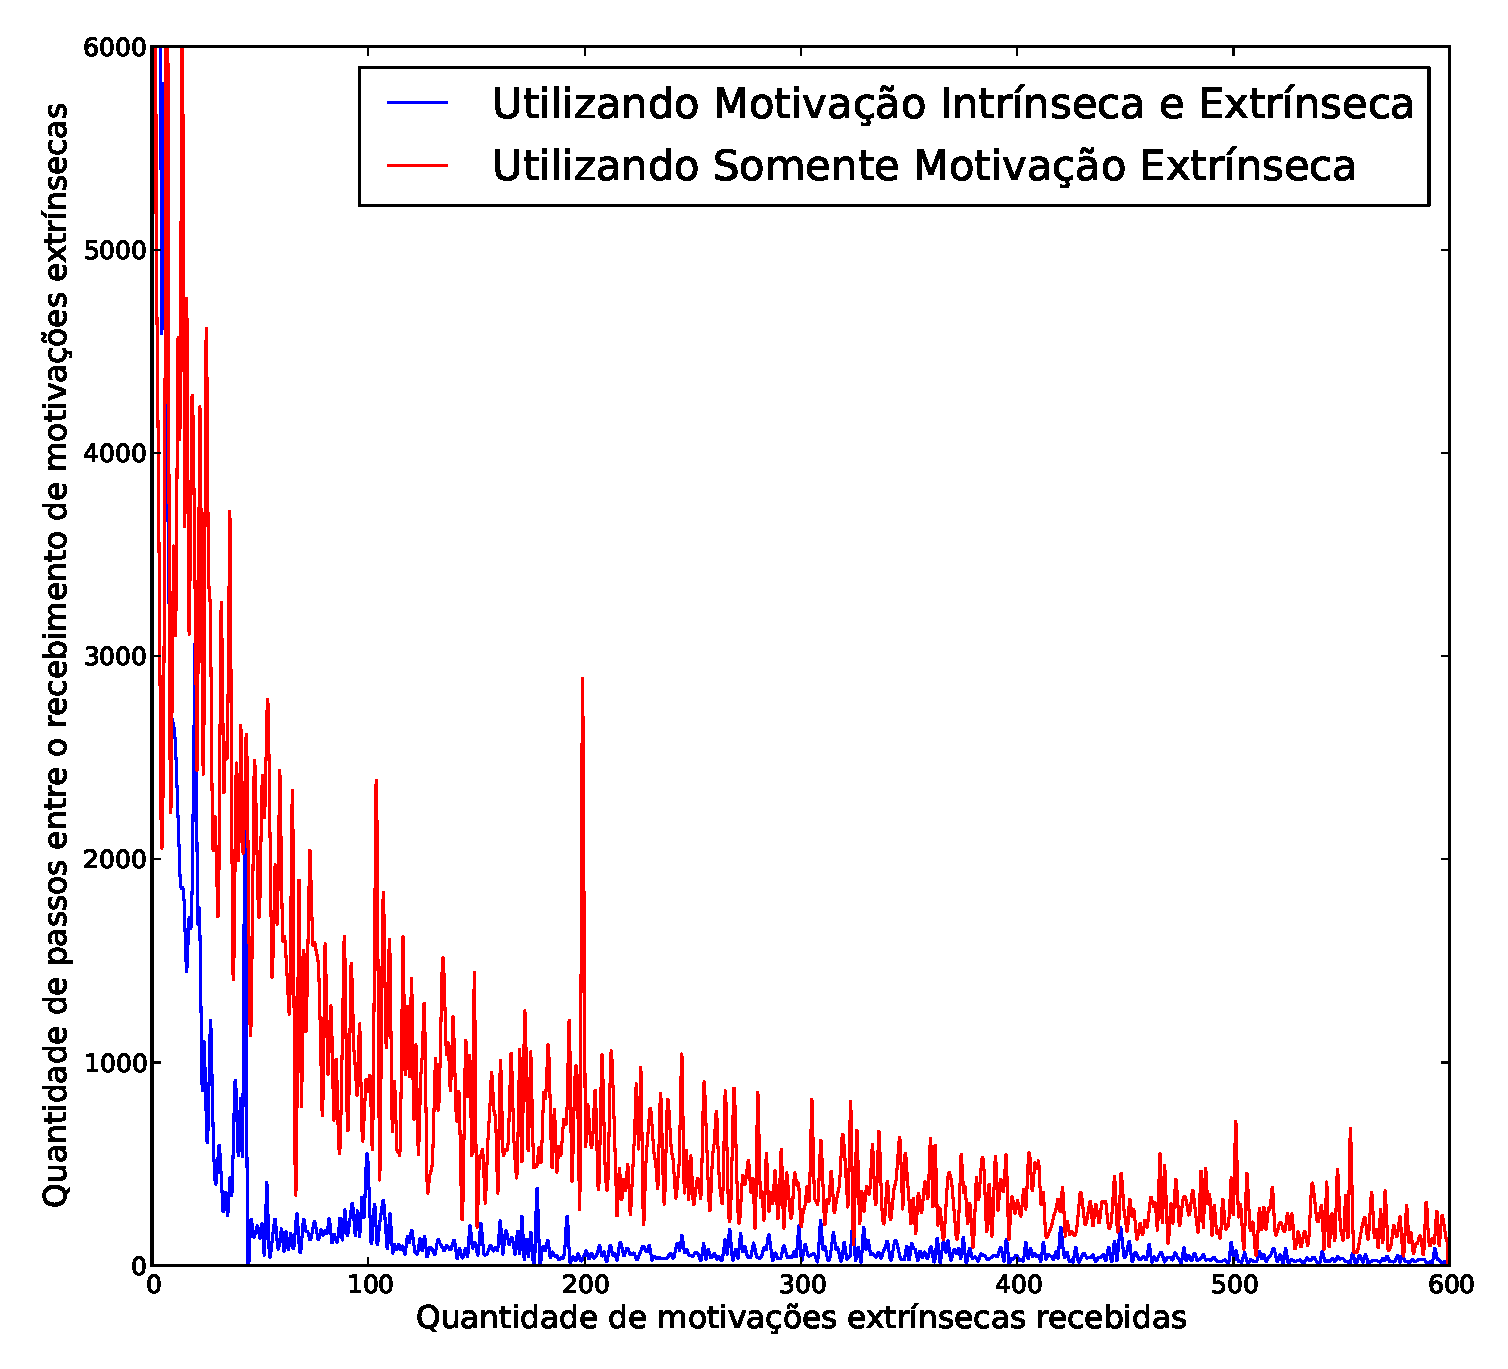
\includegraphics[width=\textwidth]{EfeitoMI}
      \caption{Efeito da Motivação Intrínseca no Aprendizado}
      \label{fig:mi}
    \end{subfigure}
    ~
    \begin{subfigure}[b]{0.47\textwidth}
      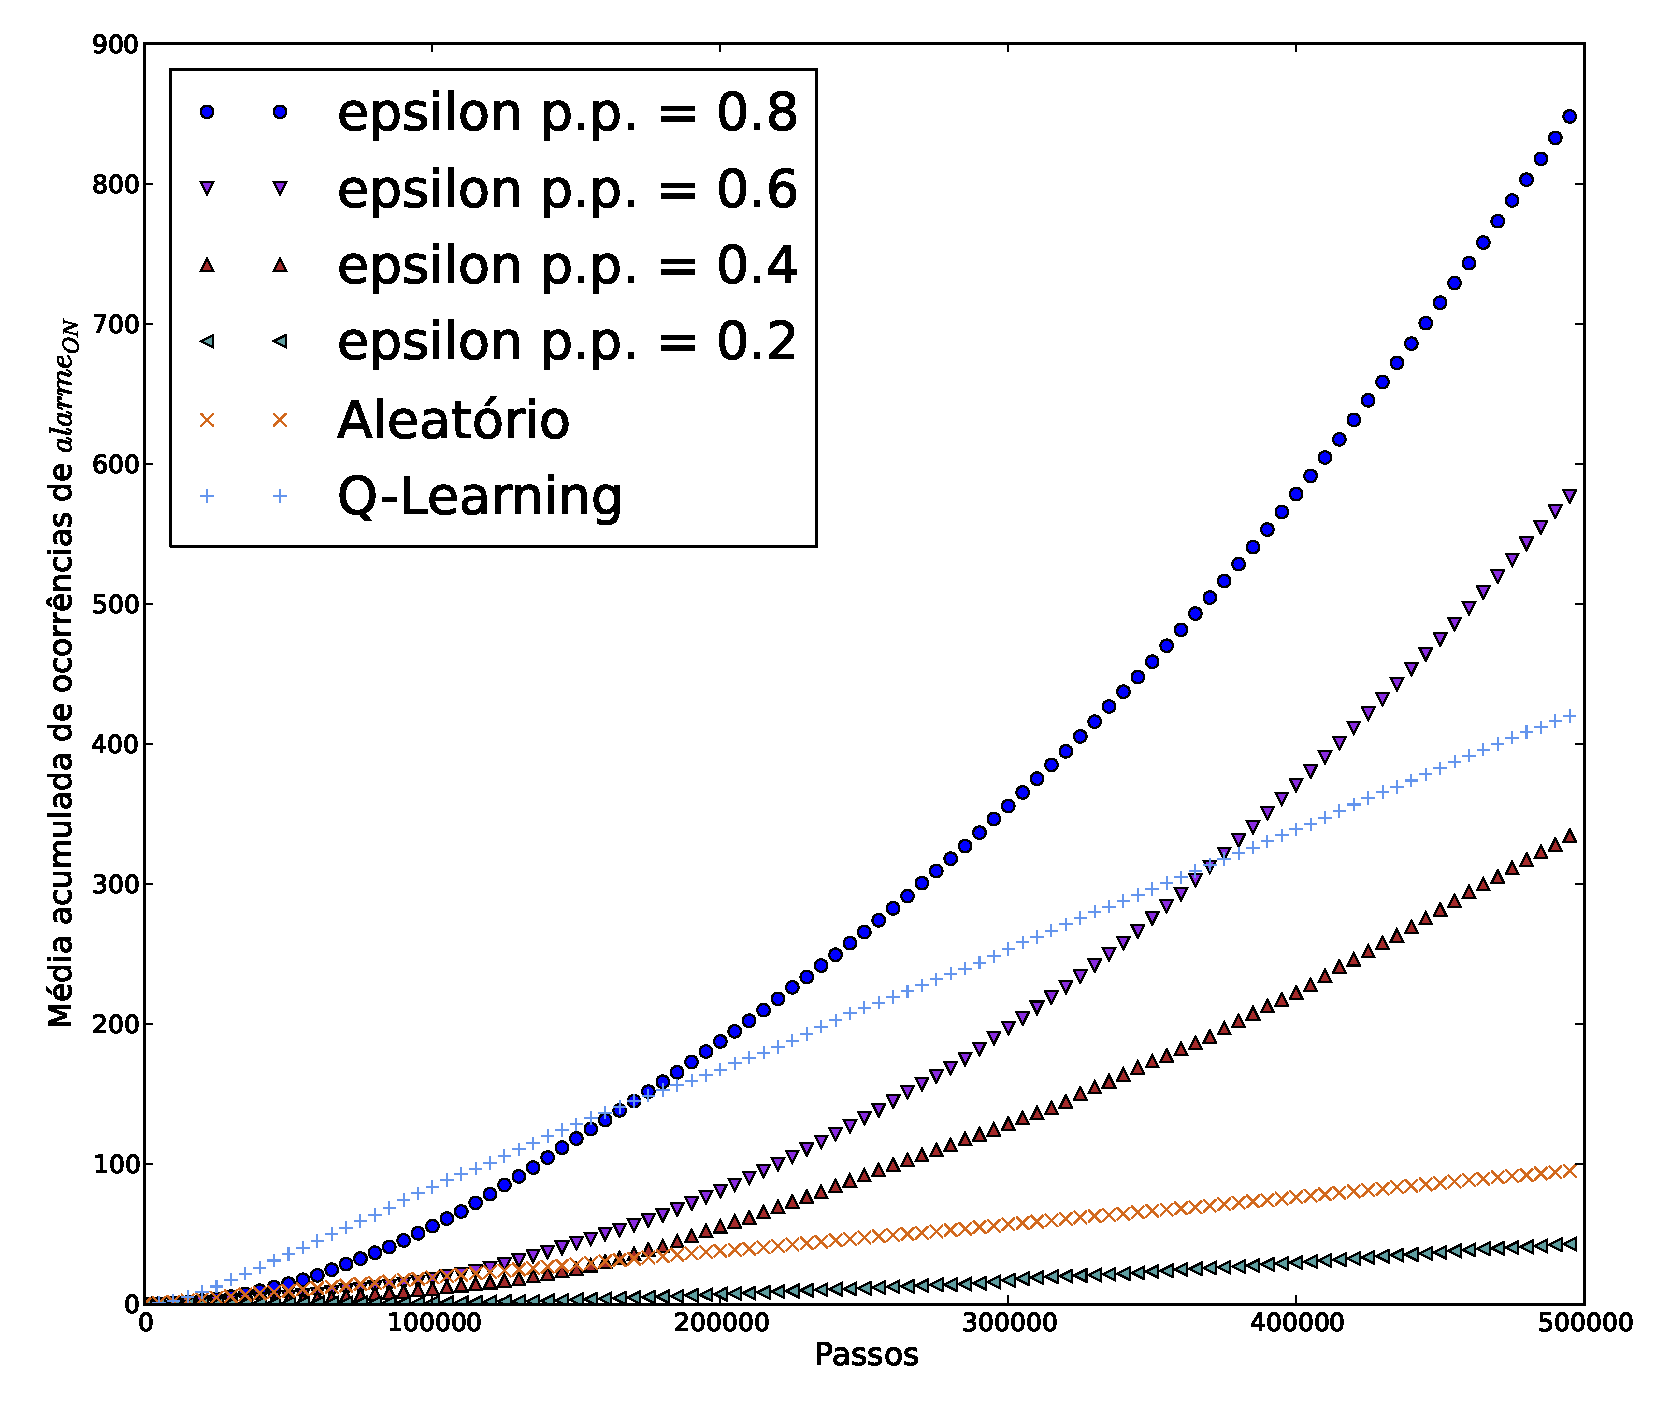
\includegraphics[width=\textwidth]{toyonxstep-mediaacum-epsopt-parcial-02-04-06-08}
      \caption{Influência de $\epsilon_{p^3}$ no Aprendizado}
      \label{fig:ep3}
    \end{subfigure}
  \end{subfigure}

  \begin{subfigure}[t]{\textwidth}
    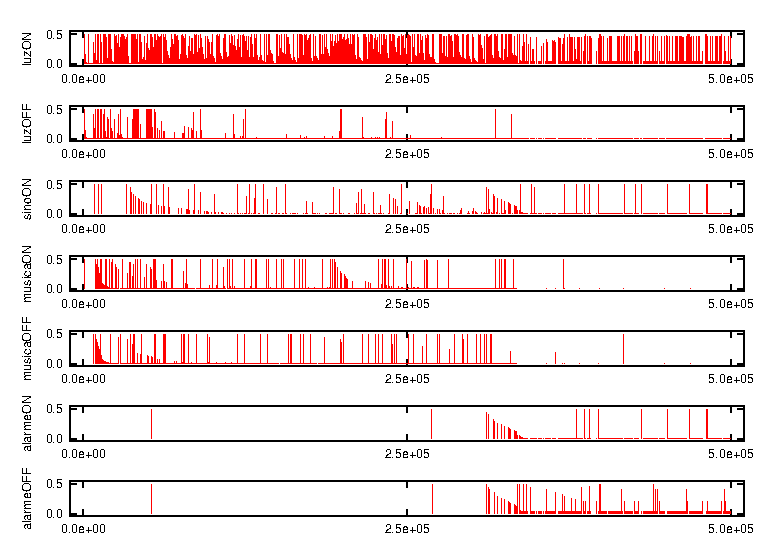
\includegraphics[width=\textwidth]{r_i-2014-07-12_07-15-03-Teri}
    \caption{Recebimento de Recompensa Intrínseca Durante o Aprendizado}
    \label{fig:ri}
  \end{subfigure}
  \caption{}\label{fig:res}
\end{figure}

% Para verificar a suscetibilidade do algoritmo proposto seria à
% \tr{estratégia de abandono da política parcial}, foram realizadas
% repetições de experimentos com variações gradativas do valor de
% $\epsilon_o$, conforme descrito na seção \tr{...}. Os resultados são
% apresentados na figura \ref{fig:epsopt}. O gráfico mostra a média
% cumulativa de ativações do \emph{monkey} por passo. Pela análise
% desses resultados, podemos verificar a variação do desempenho do
% aprendizado com o valor escolhido para $\epsilon_o$, sugerindo que a
% correta escolha desse parâmetro possui um impacto significativo no
% desempenho de aprendizado do agente. \tr{TODO: complementar}

% Foram também investigadas duas estratégias de adição de novos
% estados à política parcial: (i) \tr{backward}, em que um novo estado
% $s_t$ somente é adicionado ao conjunto iniciador $I^o$ de uma
% política parcial $o$ se ocorrer que ao realizar a transição $s_t,\
% a_t \rightarrow s_{t+1}$, tenha-se $s_{t+1} \in I^o$ e (ii)
% \tr{backward+forward}, em que ocorre a adição descrita em (i), além
% de: caso o agente, estando em $s_t \in I^o$, realizar a transição
% $s_t,\ a_t \rightarrow s_{t+1}$, $s_{t+1}$ é incluído em $I^o$. Como
% no algoritmo original, somente era realizada a adição (i), mas no
% artigo original de políticas parciais \cite{option1999} é levantada
% também a possibilidade descrita em (ii), procedeu-se à investigação
% dos possíveis resultados decorrentes dessa nova adição. Os
% resultados desse experimento podem ser vistos na figura
% \ref{fig:dummy}, que mostra \tr{...}. Pela análise dos resultados aí
% presentes, podemos concluir que \tr{...}.

% \section{Conclusão}
% Lorem ipsum dolor sit amet, consectetuer adipiscing elit. Donec
% hendrerit tempor tellus. Donec pretium posuere tellus. Proin quam
% nisl, tincidunt et, mattis eget, convallis nec, purus. Cum sociis
% natoque penatibus et magnis dis parturient montes, nascetur
% ridiculus mus. Nulla posuere. Donec vitae dolor. Nullam tristique
% diam non turpis. Cras placerat accumsan nulla. Nullam rutrum. Nam
% vestibulum accumsan nisl.

% \begin{received}
% \end{received}

% INCLUDE BIBLIOGRAPHY WHICH MUST FOLLOW kdmile.bst TEMPLATE
% \bibliographystyle{kdmile}
% \bibliography{kdmile}
% For information on how to write bibliography entries, 
% see file kdmileb.bib

\end{document}
